\section{Introduction}

\begin{wrapfigure}{r}{0.5\textwidth}
\vspace{-18pt}
\centering
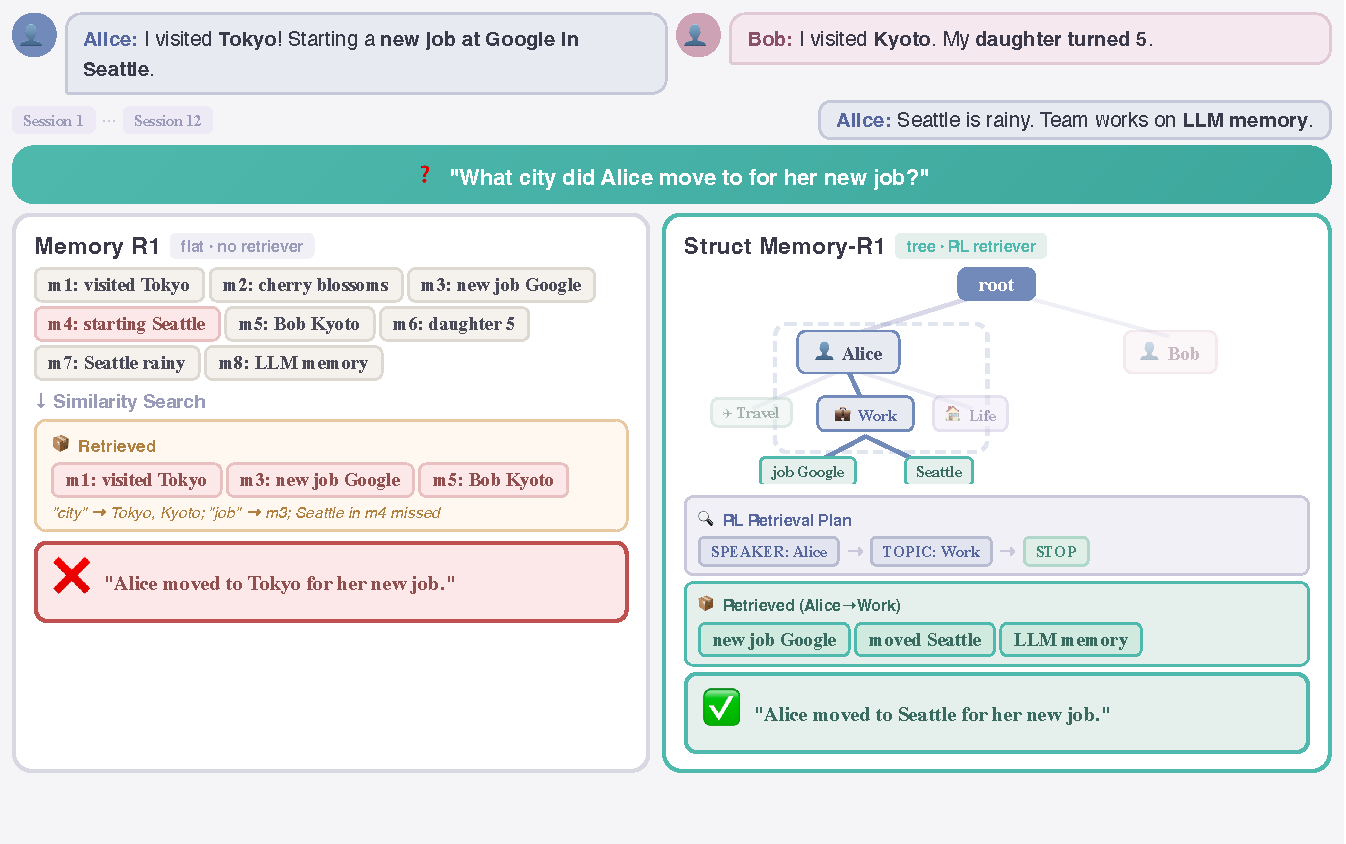
\includegraphics[width=0.5\textwidth]{figures/hook_figure.pdf}
\caption{{Motivating example.} \textbf{Memory R1} (left) uses flat similarity search, retrieving ``Tokyo'' for ``city'' but missing the job--Seattle link. \textbf{Struct Memory-R1} (right) navigates Alice $\rightarrow$ Work in the tree, correctly finding ``Seattle.''}
\label{fig:hook}
\vspace{-10pt}
\end{wrapfigure}

Memory-augmented large language models (LLMs) maintain an external memory bank that stores information from past interactions and retrieves relevant context to condition future responses~\cg{zhang2024survey}. This paradigm enables long-horizon conversational agents to access information beyond the fixed context window~\cg{maharana2024evaluating}. However, most existing memory systems represent memories as flat, unordered collections and rely on similarity-based retrieval to access them~\cg{lewis2020retrieval, khandelwal2020generalization, park2023generative}.

Flat retrieval treats all memories as independent entries in a global scoring space, ignoring the inherent relationships among them. When a user's history spans dozens of sessions covering multiple topics, events, and evolving facts, scoring each memory independently leads to \emph{retrieval interference}---semantically similar but contextually irrelevant entries compete with the correct ones. Flat update mechanisms, whether append or overwrite, similarly lack structural awareness: when a new fact arrives, the system cannot determine whether it extends an existing topic or introduces a new one. As conversations grow, these limitations compound, making consistent memory maintenance increasingly difficult.

Conversational information, however, has natural hierarchical structure: discussions revolve around people and topics, topics unfold through events and sessions, and individual facts exist within these groupings. A tree captures this hierarchy, enabling retrieval to first select a relevant branch and then read the leaves within it, and enabling updates to place new facts relative to their structural neighbors rather than into a global pool. Several prior works have explored tree-structured memory representations, including MemTree~\cg{rezazadeh2024memtree}, RAPTOR~\cg{sarthi2024raptor}, Lattice~\cg{lattice2025}, and MemWalker~\cg{chen2023memwalker}. These methods rely on heuristic or LLM-prompted approaches to construct and traverse memory hierarchies.

However, both access and update over a tree involve \emph{reasoning} through possible trajectories: the retriever must decide which branches to explore, and the writer must decide where a new fact belongs in the hierarchy (\autoref{fig:hook}). The quality of these intermediate decisions can only be judged by the correctness of the downstream answer, and direct supervision for such decisions is unavailable in standard QA data. Reinforcement learning from downstream question-answering reward is therefore the natural training signal. This follows the principle established by Search-R1~\cg{jin2025search} and Memory-R1~\cg{yan2025memory}---that information access should be trained from task outcomes---and extends it from flat memory to tree-structured access and updates.

We therefore propose \textsc{Struct Memory-R1}, a reinforcement-learning framework that learns tree-structured conversational memory from raw interaction history. \textsc{Struct Memory-R1} decomposes the problem into three coordinated components (\autoref{fig:overview}):
\begin{itemize}[nosep,leftmargin=1.5em]
\item A \textbf{Memory Manager} that receives a new turn and the current memory, then incrementally constructs and updates the memory tree through structural placement of new facts.
\item A \textbf{Retrieve Agent} that operates over the induced tree and emits an explicit search plan, selecting branches and leaves rather than relying on global flat retrieval.
\item An \textbf{Answer Agent} that reads retrieved evidence and produces the final answer.
\end{itemize}

\begin{figure}[t]
\centering
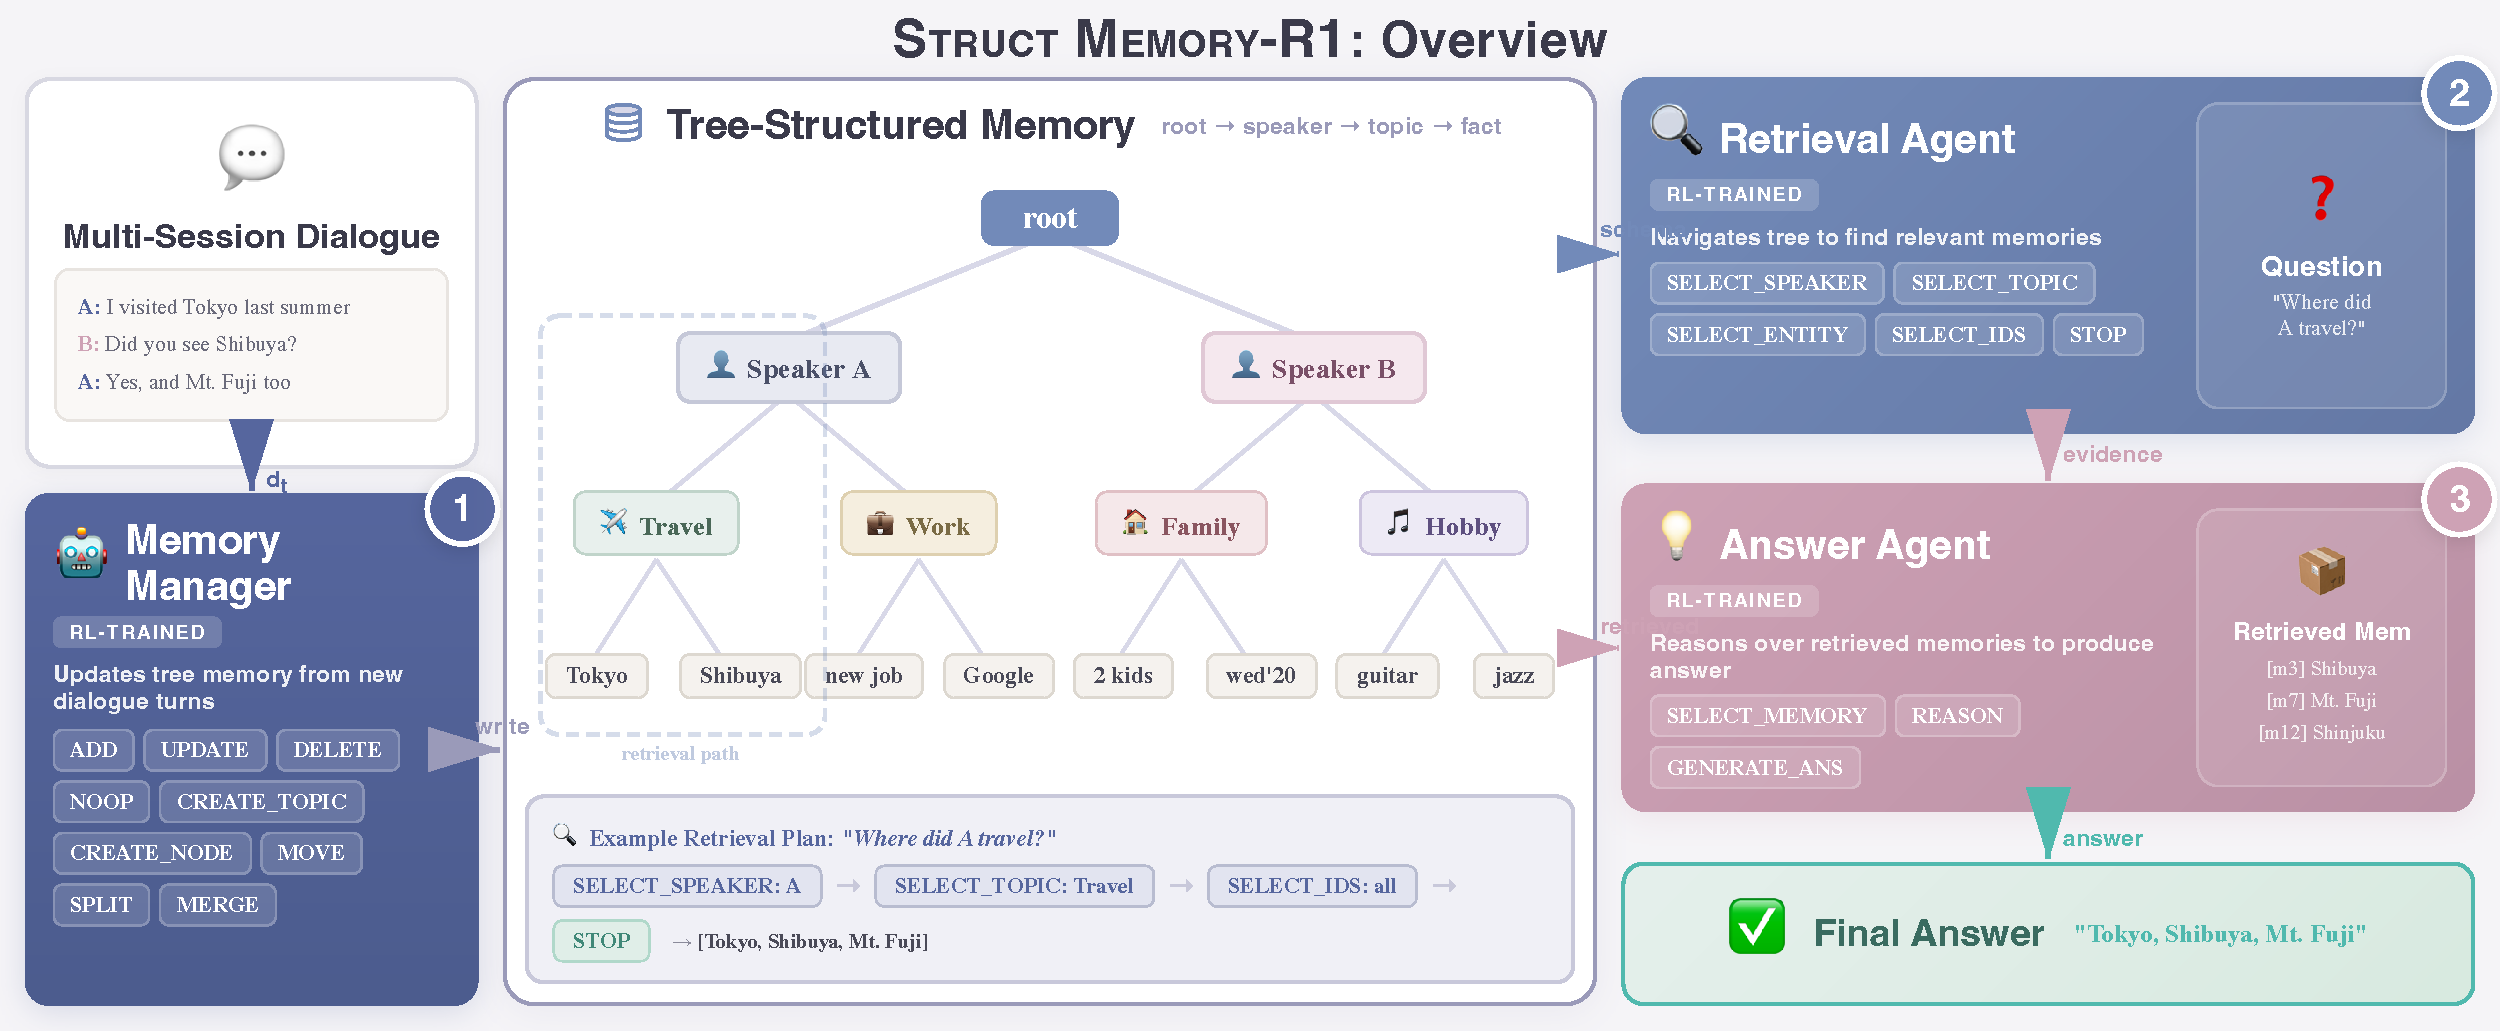
\includegraphics[width=\textwidth]{figures/struct_memory_r1_figure.pdf}
\caption{{Overview of \textsc{Struct Memory-R1}.} The Memory Manager induces and updates a tree-structured memory from raw conversation. The Retrieve Agent emits a search plan over the tree to select relevant evidence. The Answer Agent produces the final response. All three components are trained with reinforcement learning from downstream question-answering reward.}
\label{fig:overview}
\end{figure}

The decomposition follows the causal chain of the problem: the Memory Manager builds and maintains the tree, the Retrieve Agent navigates it for a given question, and the Answer Agent evaluates whether the retrieved evidence suffices. By separating these roles, \textsc{Struct Memory-R1} turns structured memory into a modular reinforcement-learning problem in which tree updates, tree access, and answering are each optimized via Group Relative Policy Optimization (GRPO) against downstream task performance.

In summary, the paper makes three contributions:
\begin{itemize}[nosep,leftmargin=1.5em]
\item We formalize the memory-augmented LLM setting and argue that conversational memory has hierarchical structure that a tree captures naturally, requiring access and update operations that differ fundamentally from those used on flat memory.
\item We propose \textsc{Struct Memory-R1}, a three-component framework that induces tree structure from raw conversation and trains tree-specific access and update policies with GRPO-based reinforcement learning.
\item We evaluate on the LoCoMo benchmark~\cg{maharana2024evaluating}, showing that tree-structured memory yields substantial gains on multi-hop (+9.0 F1) and temporal (+13.8 F1) questions while achieving the highest overall F1 among non-oracle methods.
\end{itemize}
